\section{Rotor aerodynamic and structural design} \label{sec:rotor design}
This section deals with the aerodynamic and the inner structural design of the blades for the on-shore wind turbine to be designed at the tip-speed ratio of $7.67$ and for a rotor diameter of $100.0\ m$, as decided in Section \ref{sec:system design}.

\subsection{Summary of the design}

\begin{table}[H]
\begin{center} 
\caption{Objectives and boundary conditions}\label{tab:rotordesign1}
\begin{tabular}{ |l|c| } 
\hline
\textbf{Parameter} & \textbf{Value/Description}  \\ 
\hline
Number of blades & 3  \\ 
\hline
Rotor diameter & 100.00 m \\ 
\hline
Design tip speed ratio & 7.67 \\
\hline
\end{tabular} \\
\end{center}
\end{table}

\begin{table}[H]
\begin{center} 
\caption{Objectives and boundary conditions}\label{tab:rotordesign2}
\begin{tabular}{ |l|c| } 
\hline
\textbf{Parameter} & \textbf{Value/Description}  \\ 
\hline
Aerofoil 1 & Cylinder 1  \\ 
\hline
Max. dimensionless radius r/R for aerofoil 1 & 0.11 \\ 
\hline
Aerofoil 2 & Cylinder 2 \\
\hline
Max. dimensionless radius r/R for aerofoil 2 & 0.16 \\ 
\hline
Aerofoil 3 & DU40_A17 \\
\hline
Max. dimensionless radius r/R for aerofoil 3 & 0.22 \\ 
\hline
Aerofoil 4 & DU35_A17  \\
\hline
Max. dimensionless radius r/R for aerofoil 4 & 0.33 \\ 
\hline
Aerofoil 5 & DU30_A17  \\
\hline
Max. dimensionless radius r/R for aerofoil 5 & 0.42 \\ 
\hline
Aerofoil 6 & DU25_A17  \\
\hline
Max. dimensionless radius r/R for aerofoil 6 & 0.56 \\ 
\hline
Aerofoil 7 & DU21_A17  \\
\hline
Max. dimensionless radius r/R for aerofoil 7 & 0.67 \\ 
\hline
Aerofoil 8 & NACA64_A17  \\
\hline
Max. dimensionless radius r/R for aerofoil 8 &  1\\ 
\hline
Twist offset at tip (= blade pitch angle for optimal operation) & $0.37 \deg$ \\
\hline
‘Thickness factor’ of the blade laminates & variable \\
\hline
\end{tabular} \\
\end{center}
\end{table}

\begin{table}[h]
\centering
\caption{Scaling laws used for the aerodynamic and structural design}
\label{tab:aero_struct_scaling}
\begin{tabular}{ |l|c|c| } 
\hline
\textbf{Parameter} & \textbf{Scaling Law} & \textbf{Scaling Factor}\\ 
\hline
Mass, $M$ & $R^3$ & 0.499 \\
\hline
Stiffness, $EI$ & $R^4$ & 0.397 \\
\hline
Chord, $c$ & R & 0.794\\
\hline
\end{tabular} \\
\end{table}

\begin{figure}[H]
\centering
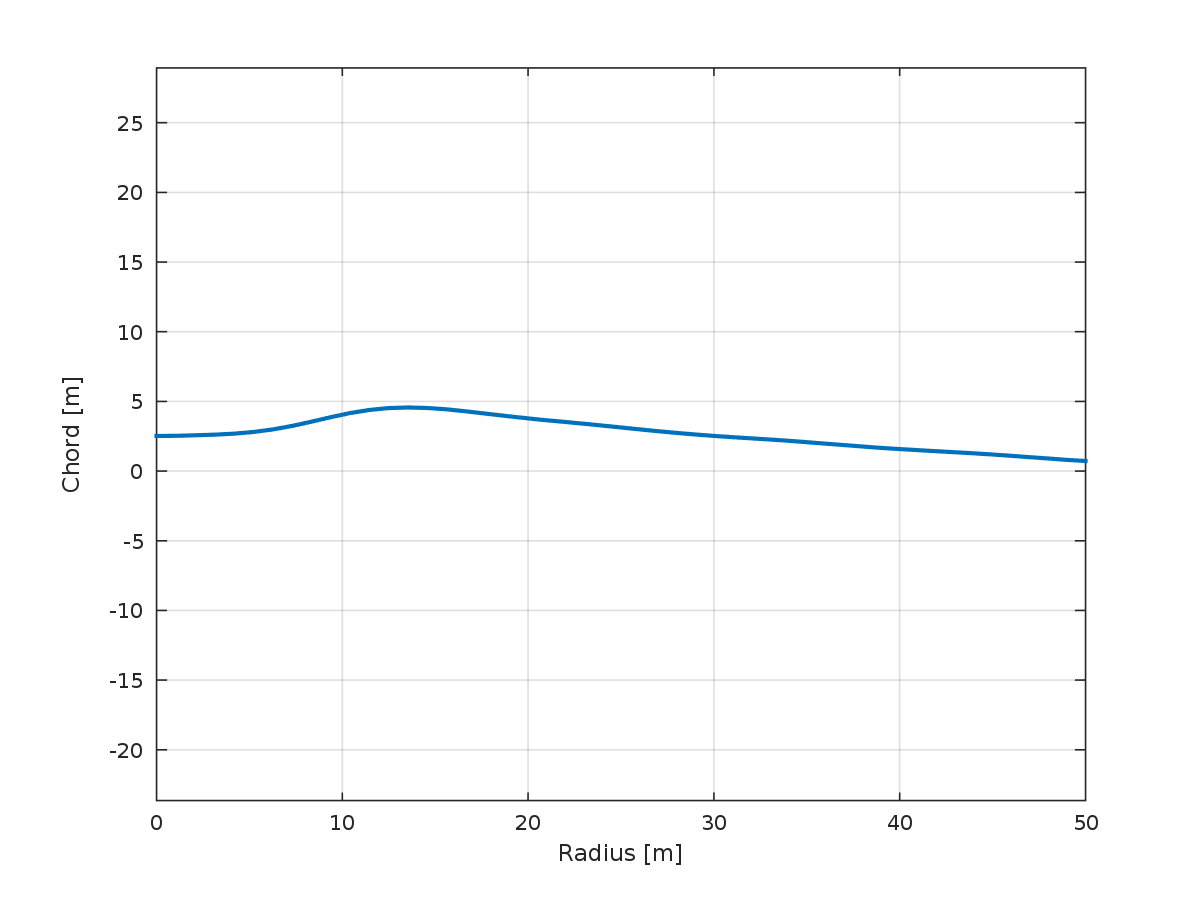
\includegraphics[width=0.7\textwidth]{Images/chord.png} 
\caption{Chord distribution}\label{fig:chord}
\end{figure}

\begin{figure}[H]
\centering
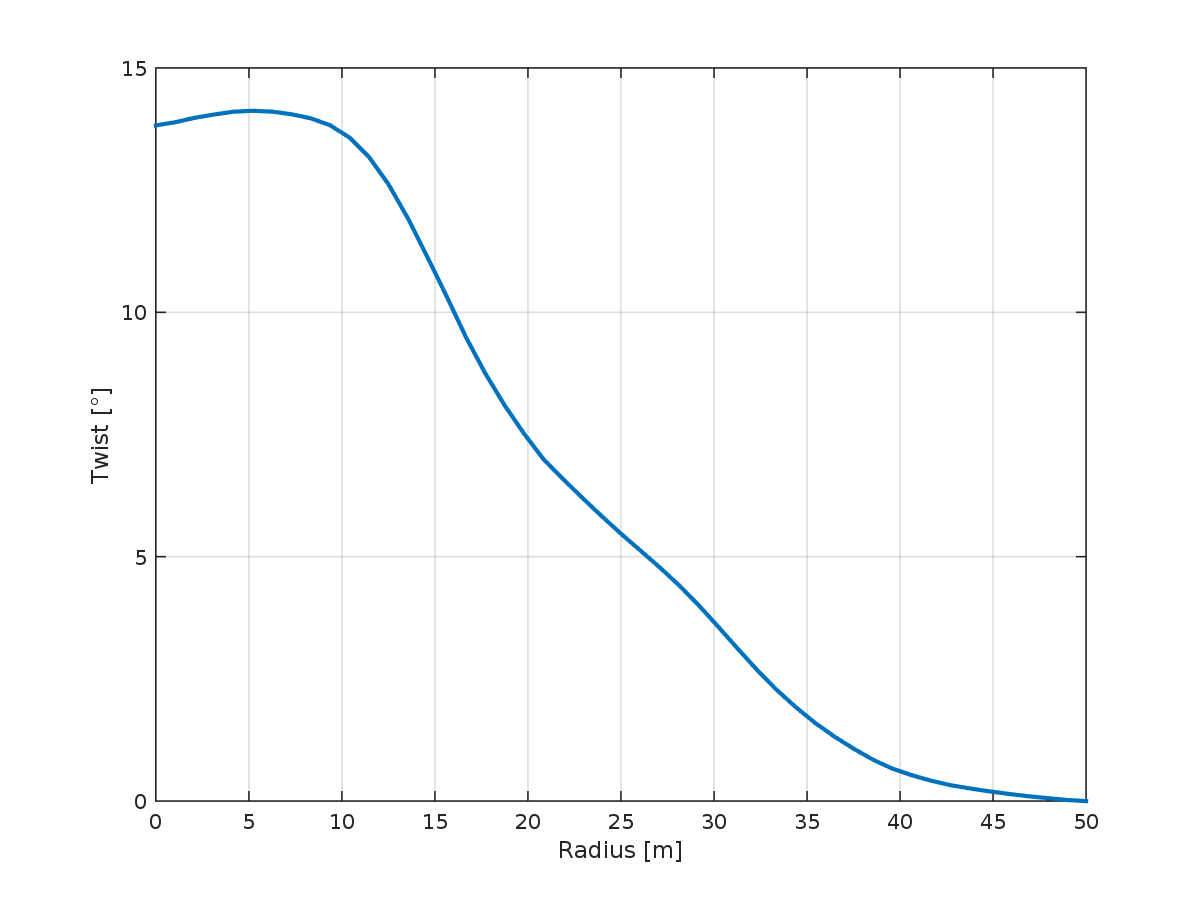
\includegraphics[width=0.7\textwidth]{Images/twist.png} 
\caption{Twist distribution}\label{fig:twist}
\end{figure}


\subsection{Supporting material, analyses and rationale}
The blade from the NREL $5\ MW$ reference turbine \cite{5MW} is designed using an optimised chord and twist distribution based on its design parameters. The design is then compared with the original reference turbine.

The blade is scaled using the scaling laws from the NREL $5\ MW$ to the desired $2\ MW$ wind turbine. The scaling laws used for each of the parameters is shown in Table \ref{tab:aero_struct_scaling}. These scaling laws are provided with the course material \cite{scaling_laws} and are based on Galileo's square-cube law which states that when an object increases in size, the area scales as square of the length specifier and volume scales as cube of the length specifier \cite{galileo}. The blade's geometry is then optimised to obtain the best desirable performance measured by maximising the power coefficient $C_p$, as can be seen in the Matlab code for task 3.

The optimisation's target is to obtain the twist and chord distribution functions that produce the highest $C_p$ under some logical constraints, i.e. the fact that the chord can not assume negative values. Moreover, a set of technological constraints are added, such that the new values can't be larger than double the original value. 

Such functions are expressed by using a set of degrees of freedom, which represent the values of twist and chord at certain uniformly distributed radial locations. The values at all the other locations are obtained by means of cubic spline interpolation. The radial locations used to evaluate the value of $C_p$ are linearly scaled from the reference NREL $5\ MW$ turbine. The value of $C_p$ is computed by using the BEM code available in the FAST program. Such code has been extracted and isolated as a function that returns the value of $C_p$ given the properties of the wind turbine, as can be seen in the Matlab code for task 3.

In order to simplify the analysis, it is decided not to change the airfoil distribution of the reference turbine. Albeit reductive, such choice has been taken to reduce the number of degrees of freedom of the problem, and because of the fact that such a discontinuous function would not be easily optimised by high performance algorithms, which usually require the computation of the Jacobian matrix of the cost function.

After the initial setup of the problem, the new values of twist, chord and overall pitch of the blade are computed by an interior-point optimisation algorithm. The results of such optimisation are smoothed out to account for technological constraints. The final value of $C_p$ is equal to $0.5005$, against an initial value of $0.48$ for the reference turbine, leading to a $4\%$ increment.

The scaled and optimised values of twist and chord are visible in figure \ref{fig:twist_and_chord}.

\begin{figure}[H]
\centering
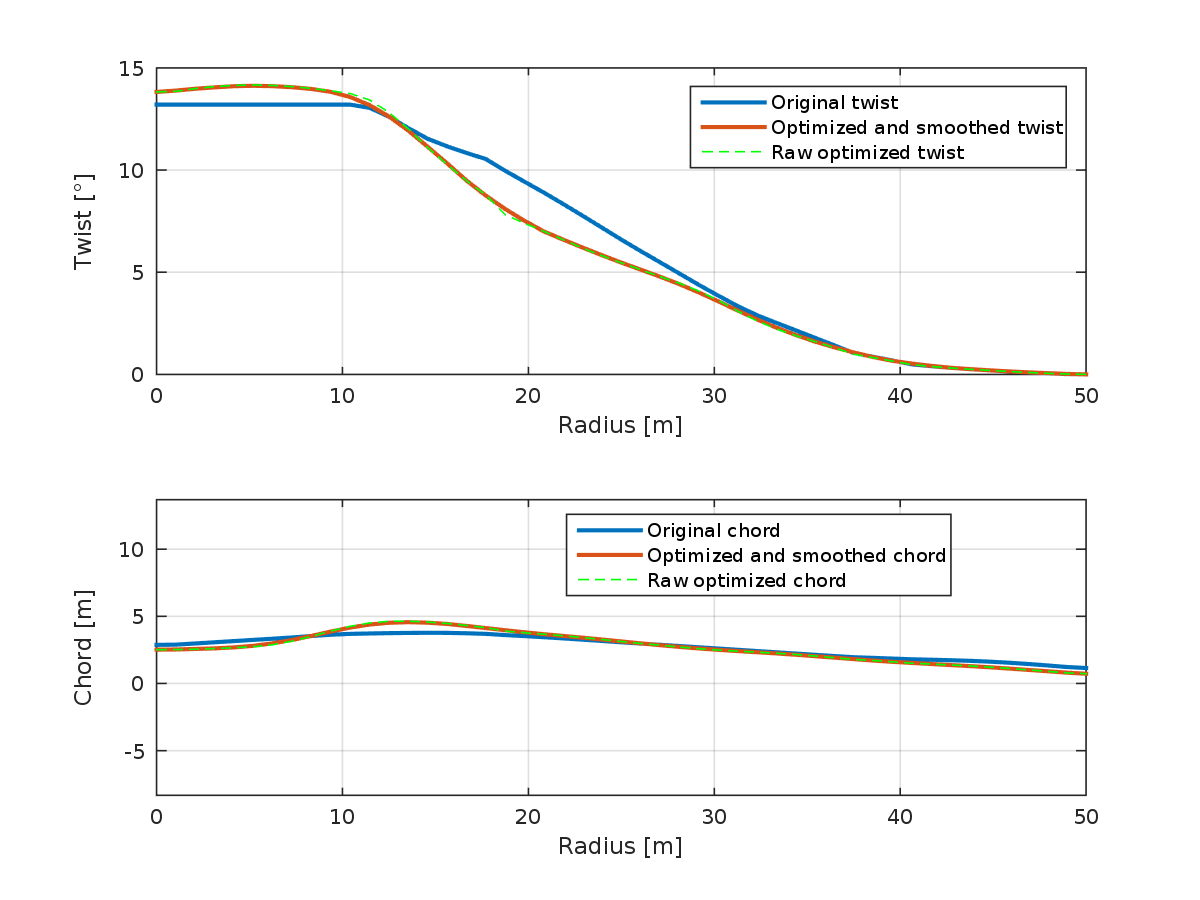
\includegraphics[width=0.7\textwidth]{Images/twist_and_chord.png} 
\caption{Twist and Chord distribution}\label{fig:twist_and_chord}
\end{figure}

The new chord is greater near the root of the blade, which is in good correlation with the theoretical distribution, which would require an infinitely large chord at the very root of the blade. At the tip of the blade, however, the chord is smaller than the original one. Such a result does not appear to have an easy physical interpretation, but it is decided to accept the results of the optimisation, because of the fact that the overall geometry of the blade is not change but a significant amount. 
The new twist of the blade appears to follow more closely the airfoil distribution, in the sense that sharper variations in the behaviour of the distribution function can be noted where the airfoil type is changed along the blade. The value of twist close to the root of the blade has not been kept constant like in the reference rotor, because of the fact that such a value has no practical effect on the aerodynamics of the blade.


The outer geometry of a rotor blade is thus defined. In order to obtain the interior structure the mass and stiffness of the blades, which make up the structural properties, are scaled from the NREL $5\ MW$ reference turbine using the scaling laws shown in Table \ref{tab:aero_struct_scaling}. The scaled blade structural properties are utilised to calculate the tip deflection of the blade designed for the new $2 MW$ wind turbine. In order to calculate the tip deflections both the reference blades and the optimised blades were loaded at a wind speed $v=9.84\ m/s$, which is the rated wind speed for the $2\ MW$ wind turbine. The tip deflection is calculated using a simple finite element model. The model is based on the Bernoulli beam theory which is applied to the blade modelled as a cantilever beam\cite{Bispl}. The blade discretized using the beam theory is shown in Figure \ref{fig:beam_theory}.

\begin{figure}[H]
\centering
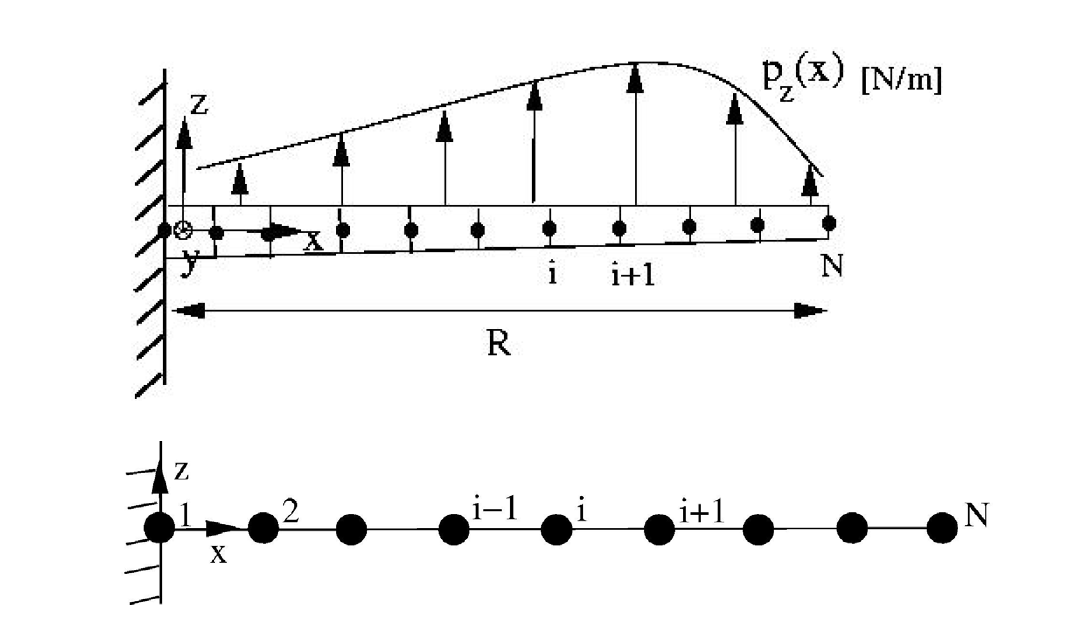
\includegraphics[width=0.8\textwidth]{Images/beam_theory.PNG} 
\caption{Discretization of the blade using classical beam theory \cite{DTU_hansen}}\label{fig:beam_theory}
\end{figure}

The equations for moment and deflection obtained from the Beam theory are applied for each section. Upon using the model, the deflections in the flap-wise and the edgewise direction are shown in Figure \ref{fig:deflection}.

\begin{figure}[H] 
\hspace*{-2.cm}
\centering
\begin{subfigure}{0.60\textwidth}
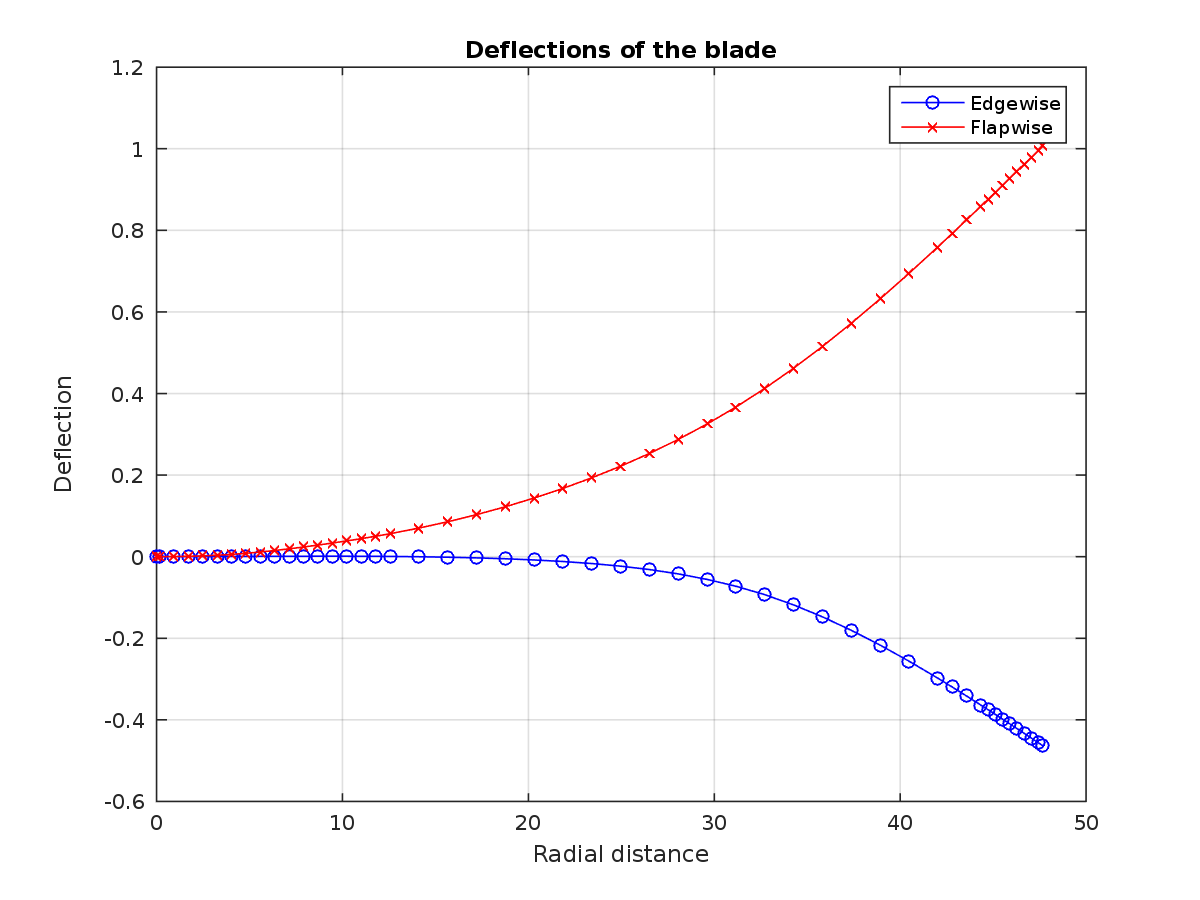
\includegraphics[width=\linewidth]{Images/deflection_optimal_no_correction.png} 
\caption{Optimised Blade}
\label{fig:deflection_optimal_1}
\end{subfigure}~
\begin{subfigure}{0.60\textwidth}
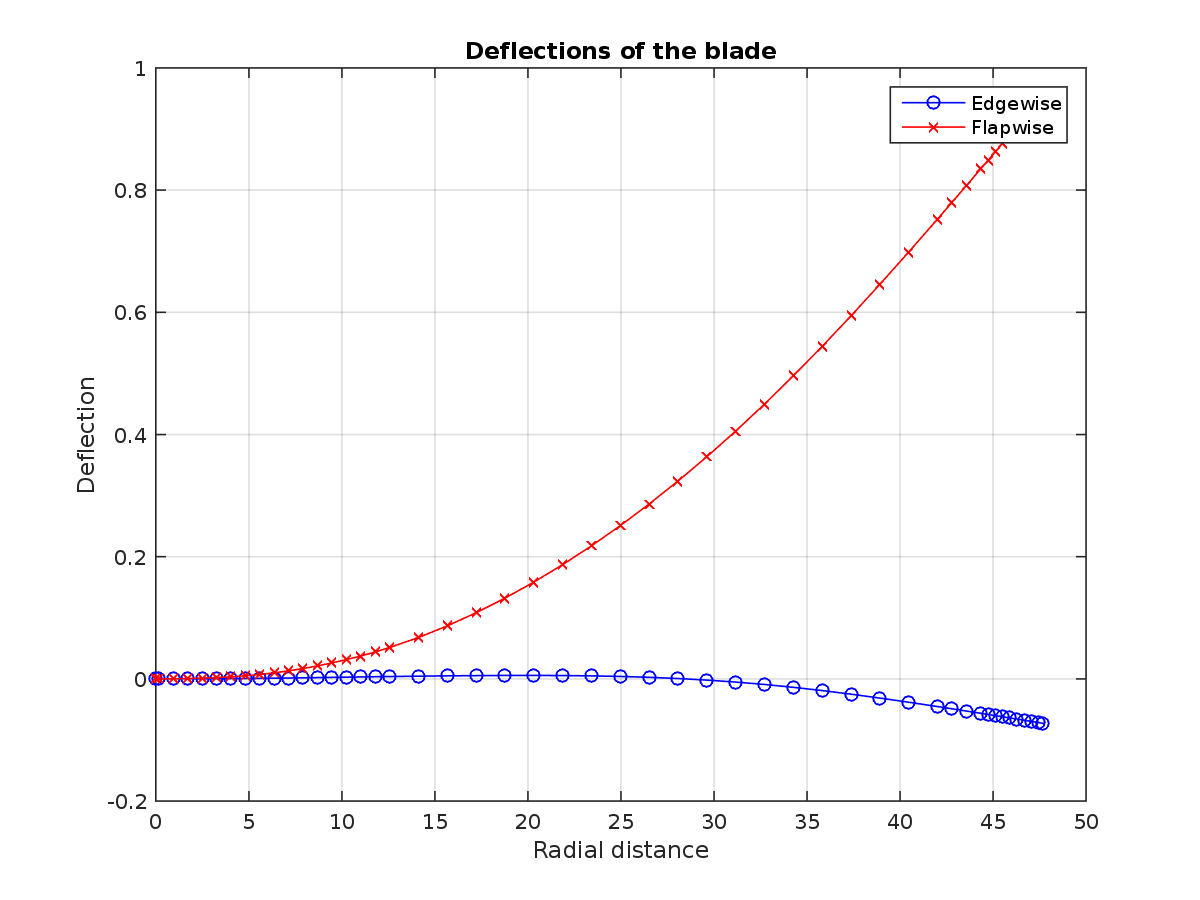
\includegraphics[width=\linewidth]{Images/deflection_scaled.png}
\caption{Scaled from Reference blade}
\label{fig:deflection_scaled}
\end{subfigure}
\caption{Deflection observed in rotor blades}
\label{fig:deflection}
\end{figure}


It can be observed from the plots shown in Figure \ref{fig:deflection} that the deflections for the new blade are smaller than that for the reference blade in the flap-wise direction. They are however seen to have increased in the edgewise direction. This is due to the differences in the chord and twist distribution observed between the optimised and the scaled reference blades, as shown in Figure \ref{fig:twist_and_chord}. The new chord and twist distributions in the optimised blade cause a redistribution in the inertia in the flap-wise and edgewise directions. Thus, the deflections in the flap-wise and edgewise directions change as a consequence. A comparison between the deflections in the edgewise and flap-wise directions that highlight this observation is shown in Figure \ref{fig:deflection_compare}.

\begin{figure}[H] 
\hspace*{-2.cm}
\centering
\begin{subfigure}{0.60\textwidth}
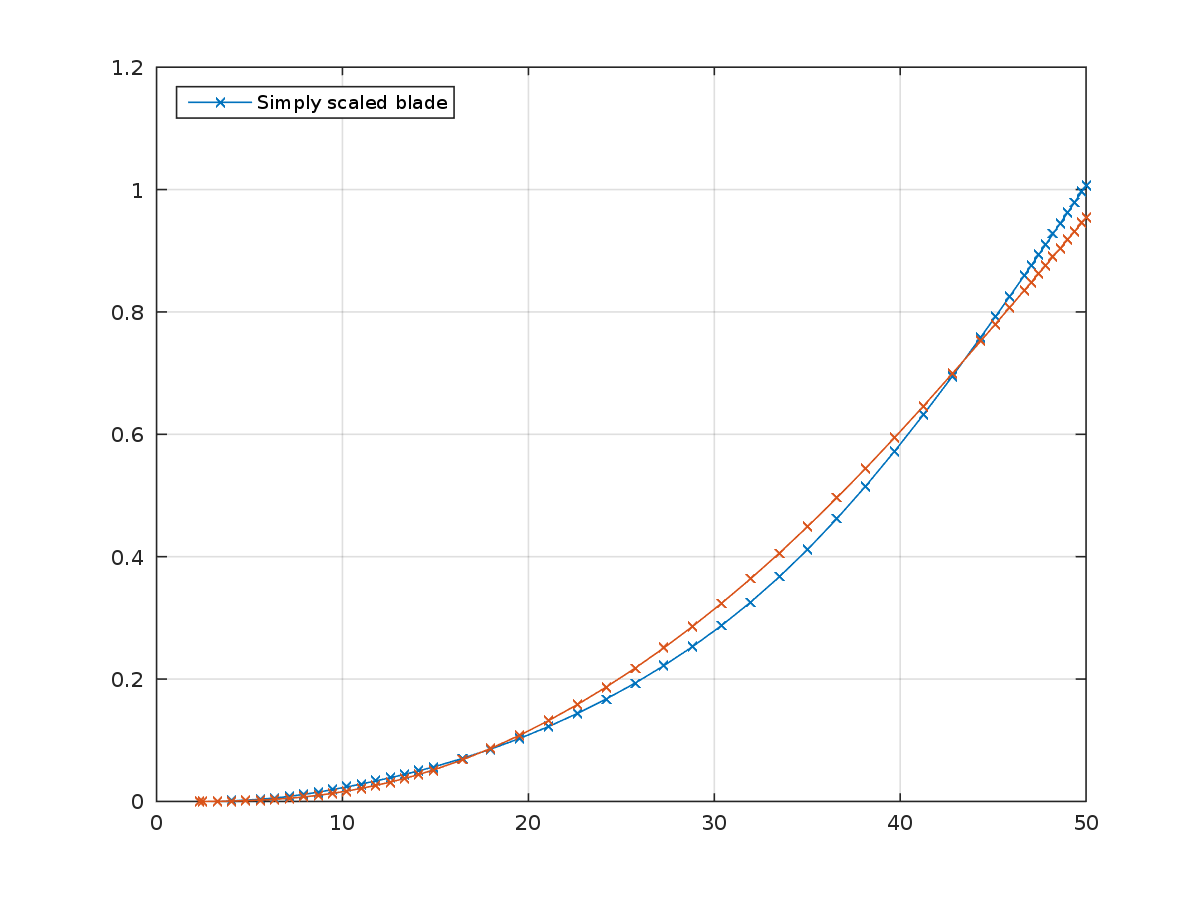
\includegraphics[width=\linewidth]{Images/edgewise_comparison.png} 
\caption{Flap-wise Deflection}
\label{fig:deflection_edge_compare}
\end{subfigure}~
\begin{subfigure}{0.60\textwidth}
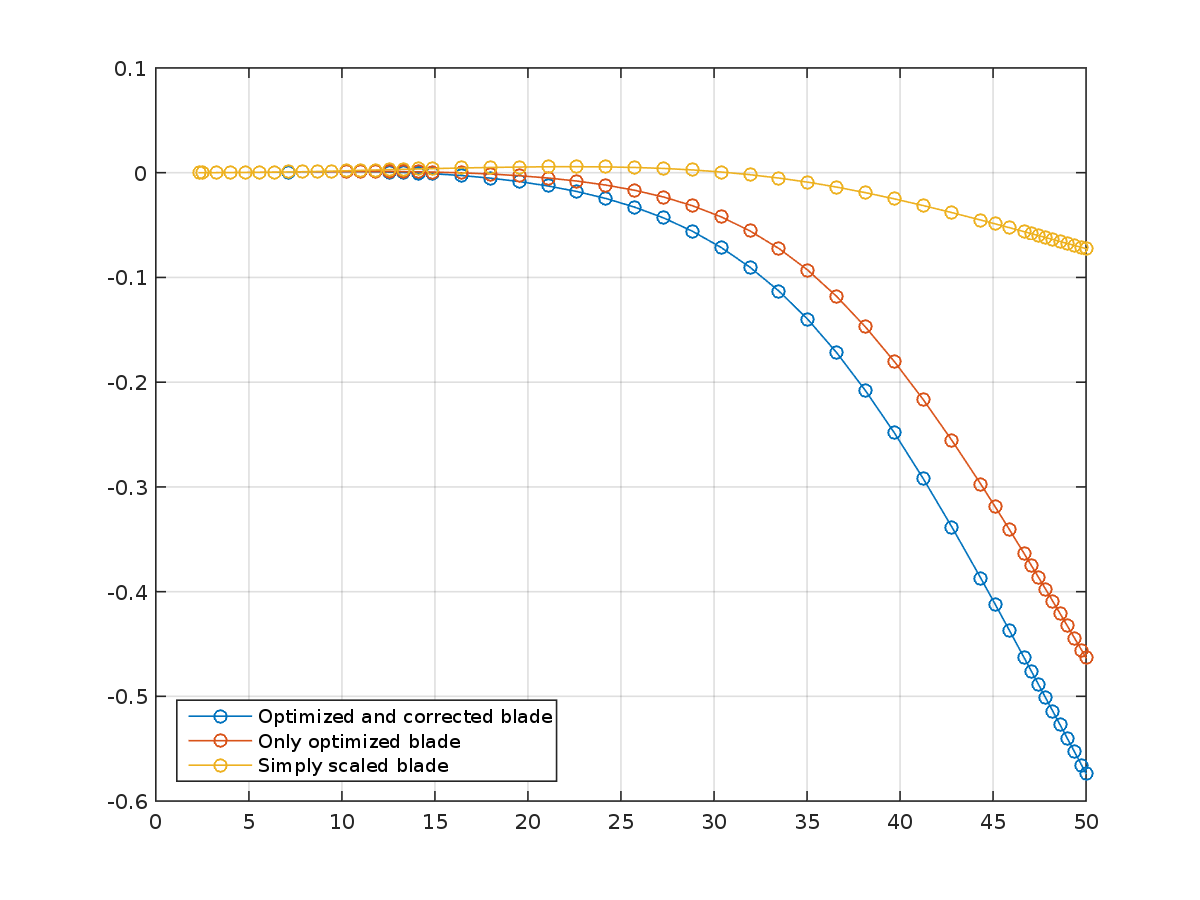
\includegraphics[width=\linewidth]{Images/flapwise_comparison.png}
\caption{Edgewise Deflection}
\label{fig:deflection_flap_compare}
\end{subfigure}
\caption{Comparison of deflections observed in the scaled reference blade and the optimised blade}
\label{fig:deflection_compare}
\end{figure}

The stresses developed in the flap-wise and edgewise directions in the $5\ MW$ reference and $2\ MW$ optimised AlphaWind turbine are compared relatively by making use of their ratios. The properties that the stresses depend on are namely, the mass $M$ and the stiffness $EI$ along the direction being considered. An additional scaling factor used is the chord $c$ of the respective blades. The chord is utilised to factor in the relative changes in the sizes of the blade cross-sections. The dependence of the stresses for the reference and optimised blades on these factors are expressed as
\begin{align}
    \sigma_{ref} &\propto \dfrac{M_{ref}}{EI_{ref}}\cdot c_{ref} \label{eq:stress_ref} \\
    \sigma_{opt} &\propto \dfrac{M_{opt}}{EI_{opt}}\cdot c_{opt} \label{eq:stress_opt}
\end{align}

where, $\sigma_{ref},\ M_{ref},\ EI_{ref}$ and $c_{ref}$ represent the stress, mass, stiffness and the chord respectively of the reference blade for the  $5\ MW$ turbine. Similarly, $\sigma_{opt},\ M_{opt},\ EI_{opt}$ and $c_{opt}$ represent the stress, mass, stiffness and the chord respectively of the optimised blade for the  $2\ MW$ turbine being designed. The relationship between the two stresses is established by taking the ratio between Equation \ref{eq:stress_opt} and Equation \ref{eq:stress_ref} and is expressed as

\begin{equation}
     \zeta = \dfrac{\sigma_{opt}}{\sigma_{ref}} = \dfrac{M_{opt}}{M_{ref}}\cdot\dfrac{EI_{ref}}{EI_{opt}}\cdot \dfrac{c_{opt}}{c_{ref}}
\label{eq:stress_ratio}
\end{equation}

The stress ratio shown in Equation \ref{eq:stress_ratio} is calculated for both edgewise, $\zeta_y$, and flap-wise, $\zeta_z$, directions. The variation of the stress ratio with the span of the blade is shown in Figure \ref{fig:stress_ratio_before}.

\begin{figure}[H]
\centering
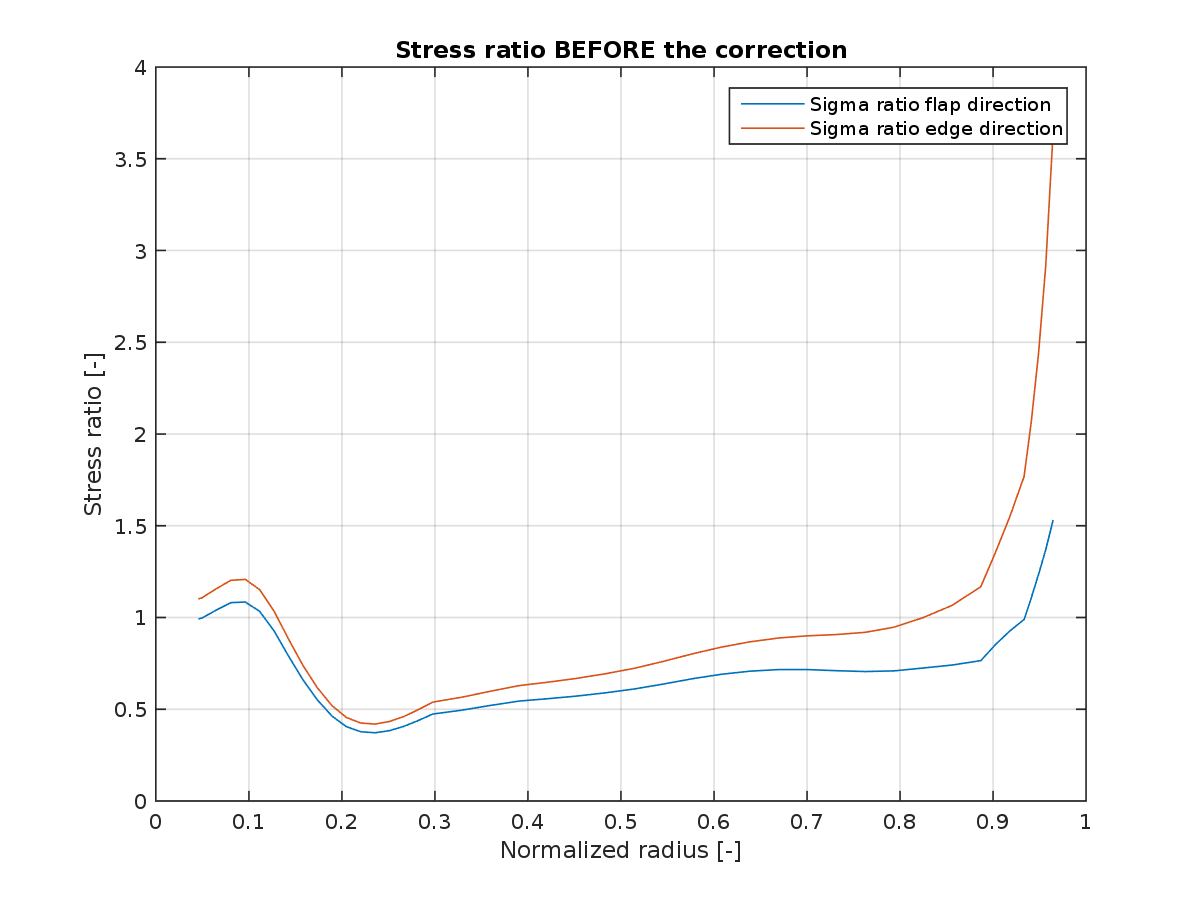
\includegraphics[width=0.7\textwidth]{Images/sigma_ratio_before.png} 
\caption{Stress ratio, $\zeta$, along the blade span  }\label{fig:stress_ratio_before}
\end{figure}

In Figure \ref{fig:stress_ratio_before} the stress ratio for both the edgewise and flap-wise directions can be seen to increase towards the tip. This means that, in the optimised blade the stresses tend to increase towards the tip as compared to the scaled reference blade. Thus, a correction factor is introduced which redistributes the inertia of the blade structure such that the more of the stress is handled by the structure near the root than by the part of the blade near the tip. The correction factor is expressed as the maximum of the stress ratio in the flap-wise and edgewise directions

\begin{equation}
     cf = max(\zeta_{z},\zeta_{y})
\label{eq:correction_factor}
\end{equation}
\\
The correction factor is then utilised to change the mass and stiffness of the blade. The new expressions for the structural properties thus become

\begin{align}
     M  &= M_{old} \cdot \sqrt{cf} \label{eq:new_mass} \\
     EI &= EI_{old} \cdot cf \label{eq:new_stiffness}
\end{align}
\\
The deflections and the stress ratios in the flap-wise and edgewise directions are then recalculated based on the new values for the structural properties obtained in Equation \ref{eq:new_mass} and Equation \ref{eq:new_stiffness}. The deflections obtained after the correction is shown in Figure \ref{fig:deflection_after}. It can be observed that when compared to the blade in Figure \ref{fig:deflection_optimal_1} the deflections in both edgewise and flap-wise directions have  increased near the tip. This is expected, due to the redistribution of the inertia from the area around the root to near the tip.

\begin{figure}[H]
\centering
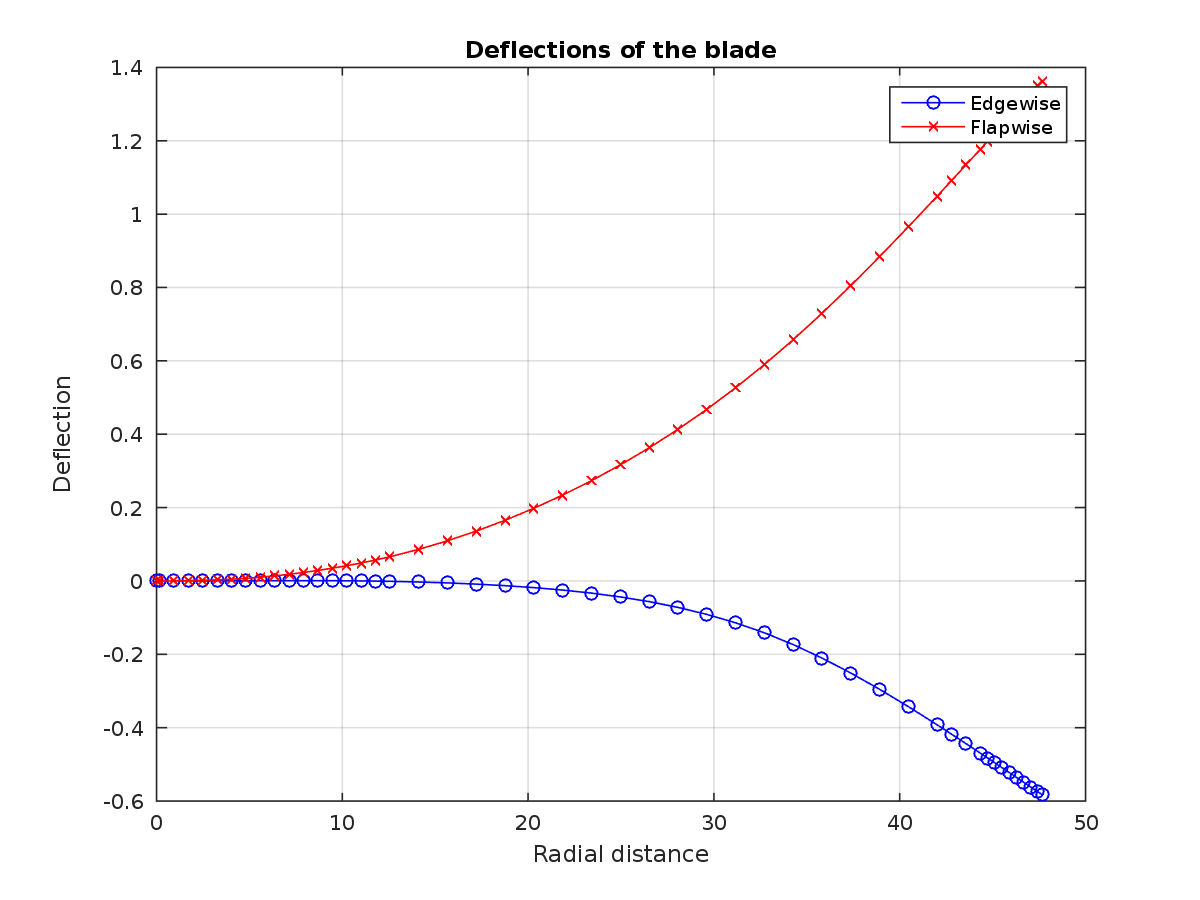
\includegraphics[width=0.7\textwidth]{Images/deflection_optimal_corrected.png} 
\caption{Deflection along the blade span after correction}
\label{fig:deflection_after}
\end{figure}

The stress distribution in the optimised blade after the correction is expressed by the stress ratio along the span of the blade shown in Figure \ref{fig:stress_ratio_after}. It is observed from the plot that the redistribution of the inertia has caused the stresses to redistribute as well. The stresses in the flap-wise direction have decreased towards the tip relative to the reference blade due to an increase in inertia. It is also seen that the stresses in the edgewise direction are found to be the same as that observed in the reference blade.

\begin{figure}[H]
\centering
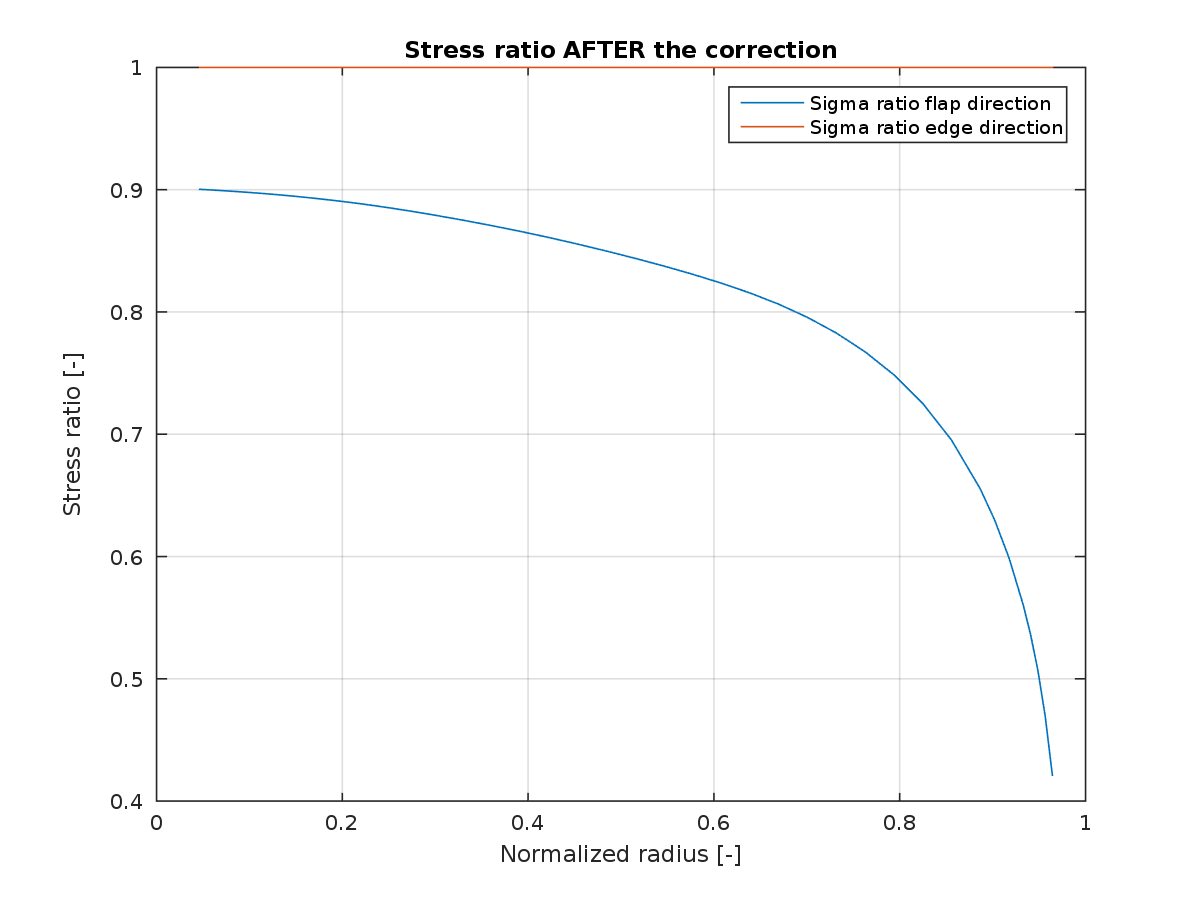
\includegraphics[width=0.7\textwidth]{Images/sigma_ratio_after.png} 
\caption{Deflection along the blade span after correction}
\label{fig:stress_ratio_after}
\end{figure}

The optimised blade after the correction of the structural properties designed for the new $2\ MW$ turbine is then utilised to calculate the power curve which is shown in Figure \ref{fig:power_curve}. The aerodynamic and structural design of the rotor is thus finalised. 